\documentclass[aspectratio=169,10pt]{beamer}

\usetheme{Madrid}
\usecolortheme{default}
\setbeamertemplate{navigation symbols}{}
\setbeamertemplate{footline}[frame number]
\setbeamertemplate{itemize items}[circle]
\setbeamertemplate{bibliography item}{\insertbiblabel}

\usepackage{iftex}
\ifPDFTeX
  \usepackage[T2A]{fontenc}
  \usepackage[utf8]{inputenc}
  \usepackage[russian]{babel}
\else
  \usepackage{fontspec}
  \setmainfont{DejaVu Serif}
  \setsansfont{DejaVu Sans}
  \setmonofont{DejaVu Sans Mono}
  \usepackage[russian]{babel}
\fi

\usepackage{amsmath,amssymb}
\usepackage{booktabs}
\usepackage{graphicx}
\graphicspath{{figs/}}
\usepackage{tikz}
\usetikzlibrary{arrows.meta,positioning,calc,decorations.pathreplacing}

\newcommand{\E}{\mathbb{E}}
\newcommand{\KL}{\mathrm{KL}}
\newcommand{\yx}{y_{1:n}\mid x_{1:n}}
\newcommand{\src}[1]{\par\vspace{2pt}{\scriptsize\color{black!55}Источник: #1\par}}

\title[Description Length of Deep Learning Models]{The Description Length of Deep Learning Models}
\subtitle{L\'eonard Blier, Yann Ollivier --- NIPS 2018}
\author{Алябушев Павел}
\institute{Bayesian multimodeling, МФТИ}
\date{2026}

\begin{document}

%% 1 ---------------------------------------------------------------
\begin{frame}
  \titlepage
\end{frame}

%% 2 ---------------------------------------------------------------
\begin{frame}{Вопрос статьи: сжимают ли данные сети с миллионами параметров?}
  \begin{itemize}
    \item Принцип MDL и теория индукции Соломонова: хорошая модель --- та, что хорошо сжимает данные \emph{без потерь}, \alert{включая стоимость описания самой модели}.
    \item Глубокие сети, на первый взгляд, противоречат принципу: параметров очень много.
    \item Свёрточные сети достигают 100\% точности на обучающей выборке даже со \emph{случайными} метками (Zhang et al., 2017).
  \end{itemize}
  \begin{block}{Что делают авторы}
    Измеряют, сколько бит нужно, чтобы без потерь передать метки обучающей выборки вместе с моделью. Новых архитектур и алгоритмов обучения не предлагают.
  \end{block}
  \begin{columns}[T]
    \begin{column}{0.5\textwidth}
      \textcolor{structure}{Вклад 1}\\
      Вариационный код (Hinton, van Camp, 1993) даёт неожиданно \alert{плохие} оценки длины, хотя прямо минимизирует длину описания.
    \end{column}
    \begin{column}{0.5\textwidth}
      \textcolor{structure}{Вклад 2}\\
      Prequential-код поверх обычного обучения даёт оценки в 2--6 раз короче вариационных и лучше согласуется с точностью на тесте.
    \end{column}
  \end{columns}
\end{frame}

%% 3 ---------------------------------------------------------------
\begin{frame}{Случайные метки не сжимаются}
  \begin{columns}[T]
    \begin{column}{0.52\textwidth}
      \centering
      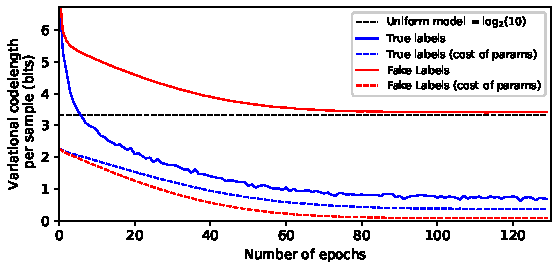
\includegraphics[width=\linewidth]{fig1_fake_labels}
    \end{column}
    \begin{column}{0.46\textwidth}
      \small
      MNIST, MLP с 3 скрытыми слоями по 200 нейронов (ReLU), вариационное обучение. По оси $y$ --- вариационная длина кода на один пример, бит.
      \begin{itemize}
        \item \textcolor{blue}{Истинные метки}: длина ниже равномерного кода $\log_2 10\approx3{,}32$ бит; около половины длины --- информация в весах.
        \item \textcolor{red}{Случайные метки}: длина сходится к равномерному коду, вклад весов $\to 0$: обучения не произошло.
      \end{itemize}
      \begin{block}{Предложение 2 (прил.~A)}
        Если $Y_1,\dots,Y_n$ равномерны на $\{1,\dots,K\}$ и независимы, то с вероятностью $\ge 1-2^{-\delta}$ \emph{любая} программа на фиксированной эталонной машине (она может зависеть от $x$, но не от $Y$) даёт $L(Y_{1:n}\mid x_{1:n})\ge n\log_2K-\delta-1$.
      \end{block}
    \end{column}
  \end{columns}
\end{frame}

%% 4 ---------------------------------------------------------------
\begin{frame}{Постановка: Алиса передаёт метки Бобу}
  \centering
  \begin{tikzpicture}[box/.style={draw,rounded corners,align=center,minimum height=0.95cm,inner sep=4pt,font=\small},
                      arr/.style={-{Stealth},thick}]
    \node[box,fill=blue!8] (a) {Алиса\\знает $x_{1:n}$ и $y_{1:n}$};
    \node[box,fill=green!8,right=6.2cm of a] (b) {Боб\\знает только $x_{1:n}$};
    \draw[arr] (a) -- node[above,font=\small]{сообщение длины $L(\yx)$ бит} node[below,font=\scriptsize]{без потерь, вместе с описанием модели} (b);
  \end{tikzpicture}

  \vspace{0.3em}
  \raggedright
  \begin{block}{Предложение 1 (код Шеннона--Хаффмана)}
    Если модель $p(y\mid x)$ заранее известна обоим, метки передаются за (с точностью до 1 бита на всю выборку)
    \[
      L_p(\yx)=-\sum_{i=1}^n\log_2 p(y_i\mid x_i)\quad\text{--- кросс-энтропия в битах.}
    \]
  \end{block}
  \begin{columns}[T]
    \begin{column}{0.5\textwidth}
      \textcolor{structure}{Равномерный код}: $L^{\mathrm{unif}}=n\log_2K$.\\
      MNIST: $60\,000\cdot\log_2 10\approx199$ кбит.\\
      CIFAR-10: $50\,000\cdot\log_2 10\approx166$ кбит.\\[2pt]
      Коэффициент сжатия $=L/L^{\mathrm{unif}}$.
    \end{column}
    \begin{column}{0.5\textwidth}
      \textcolor{structure}{Связь с взаимной информацией}\\
      Для префиксных кодов $\E_q[L]\ge H(y\mid x)$, поэтому $H(y)-\E_q[L]\le I(y;x)$: сжатие меток --- оценка $I(y;x)$ снизу. Классы почти сбалансированы, $H(y)\approx\log_2K$.
    \end{column}
  \end{columns}
\end{frame}

%% 5 ---------------------------------------------------------------
\begin{frame}{Двухчастный код: сначала веса, потом метки}
  \begin{block}{Определение 1 (two-part code)}
    \[
      L^{\text{2-part}}_{\theta^*}(\yx)=L_{\mathrm{param}}(\theta^*)-\sum_{i=1}^n\log_2p_{\theta^*}(y_i\mid x_i).
    \]
  \end{block}
  \begin{itemize}
    \item float32: $L_{\mathrm{param}}(\theta)=32\dim\theta$. Сеть с $10^6$ параметров $\Rightarrow$ 32 Мбит, примерно в 200 раз больше равномерного кода на CIFAR-10.
    \item Практическое сжатие сетей (прунинг, квантизация, Han et al., 2015) --- тот же двухчастный код с умным кодом для $\theta$. Всё равно длиннее равномерного кода.
    \item Случайное аффинное подпространство размерности $k$ (intrinsic dimension, Li et al., 2018): передаются seed и $k$ координат.
  \end{itemize}
  \begin{center}
  \small
  \begin{tabular}{lcc}
    \toprule
    Оценка снизу (только веса) & MNIST & CIFAR-10 \\
    \midrule
    float32, 2-part & $>8{,}6$ Мбит & $>428$ Мбит \\
    Network compression & $>400$ кбит & $>14$ Мбит \\
    Intrinsic dim.\ (точность 90\% / 70\%) & $>9{,}28$ кбит & $>92{,}8$ кбит \\
    \bottomrule
  \end{tabular}
  \end{center}
\end{frame}

%% 6 ---------------------------------------------------------------
\begin{frame}{Вариационный и байесовский коды}
  Веса передаются с ограниченной точностью: неопределённость $\beta$ задаёт точность передачи $\theta$; с аргументом \emph{bits-back} (Hinton, van Camp, 1993; Honkela, Valpola, 2004) это явная схема кодирования.
  \begin{block}{Определение 2 (variational code), prior $\alpha$, любое распределение $\beta$}
    \[
      L^{\mathrm{var}}_\beta(\yx)=\KL(\beta\,\|\,\alpha)-\E_{\theta\sim\beta}\Big[\sum_{i=1}^n\log_2p_\theta(y_i\mid x_i)\Big]
      \quad(=\;-\mathrm{ELBO}\text{ в битах}).
    \]
  \end{block}
  \begin{columns}[T]
    \begin{column}{0.5\textwidth}
      \textcolor{structure}{Байесовский код}
      \[
        L^{\mathrm{Bayes}}=-\log_2\!\int p_\theta(\yx)\,\alpha(\theta)\,d\theta,
      \]
      $L^{\mathrm{var}}_\beta\ge L^{\mathrm{Bayes}}$, равенство $\iff$ $\beta$ --- апостериорное распределение.
    \end{column}
    \begin{column}{0.5\textwidth}
      \textcolor{structure}{Как считали (прил.~C)}
      \begin{itemize}
        \item $\beta=\mathcal N(\mu,\mathrm{diag}\,\sigma^2)$, $\sigma_i=\log(1+e^{\rho_i})$
        \item prior $\alpha=\mathcal N(0,\sigma_0^2I)$, $\sigma_0=0{,}05$ (подобран по лучшей длине)
        \item Монте-Карло с одним сэмплом ($S=1$), библиотека Pyvarinf
      \end{itemize}
    \end{column}
  \end{columns}
\end{frame}

%% 7 ---------------------------------------------------------------
\begin{frame}{Prequential (онлайн) код: веса не передаются вовсе}
  \centering
  \begin{tikzpicture}[x=1cm,y=1cm]
    \def\h{0.55}
    \fill[black!15] (0,0) rectangle (0.7,\h);
    \foreach \a/\b/\c in {0.7/1.4/blue!12, 1.4/2.8/blue!20, 2.8/5.6/blue!28, 5.6/11.2/blue!36}
      \fill[\c] (\a,0) rectangle (\b,\h);
    \foreach \x in {0,0.7,1.4,2.8,5.6,11.2} \draw (\x,0) -- (\x,\h);
    \draw (0,0) rectangle (11.2,\h);
    \node[below,font=\scriptsize] at (0,0) {$1$};
    \node[below,font=\scriptsize] at (0.7,0) {$t_1$};
    \node[below,font=\scriptsize] at (1.4,0) {$t_2$};
    \node[below,font=\scriptsize] at (2.8,0) {$t_3$};
    \node[below,font=\scriptsize] at (5.6,0) {$t_4$};
    \node[below,font=\scriptsize] at (11.2,0) {$n$};
    \node[font=\scriptsize,align=center,below=10pt] at (0.35,0) {равно-\\мерно};
    \draw[decorate,decoration={brace,amplitude=4pt}] (0,\h+0.08) -- (2.8,\h+0.08)
      node[midway,above=5pt,font=\scriptsize,blue!50!black] (tr) {обучаем $\hat\theta_{t_3}$ на $[1;t_3]$};
    \draw[-{Stealth},thick,blue!70!black] (2.3,1.1) .. controls (3.3,1.45) and (4.0,1.3) .. (4.2,\h+0.05);
    \node[font=\scriptsize,blue!50!black,anchor=west] at (4.5,0.95) {кодируем им блок $(t_3;t_4]$, затем переобучаем на $[1;t_4]$, \dots};
  \end{tikzpicture}

  \raggedright
  \begin{block}{Определение 3 (prequential code), алгоритм 2}
    \[
      L^{\mathrm{preq}}(\yx)=t_1\log_2K+\sum_{s=1}^{S-1}-\log_2p_{\hat\theta_{t_s}}\big(y_{t_s+1:t_{s+1}}\mid x_{t_s+1:t_{s+1}}\big).
    \]
  \end{block}
  \begin{itemize}
    \item Боб сам обучает ту же модель на уже декодированных метках. Заранее согласуют модель, алгоритм обучения, гиперпараметры и seed $\omega$.
    \item $L^{\mathrm{preq}}$ минус log-loss финальной модели на тех же обучающих данных --- сколько информации о данных хранят обученные веса (по авторам).
    \item Блоки удваиваются: $t_s=8,16,\dots,32768$ (MNIST), $10,20,\dots,40960$ (CIFAR-10); последний блок --- до $n$.
  \end{itemize}
\end{frame}

%% 8 ---------------------------------------------------------------
\begin{frame}{Как ставили эксперименты}
  \begin{columns}[T]
    \begin{column}{0.5\textwidth}
      \textcolor{structure}{Данные}: MNIST ($n=60\,000$) и CIFAR-10 ($n=50\,000$), $K=10$. Передаются метки обучающей выборки; точность меряется на тесте.

      \medskip
      \textcolor{structure}{Вариационный код}: перебор полносвязных и свёрточных сетей; лучшими оказались небольшие сети (LeNet-подобные).
    \end{column}
    \begin{column}{0.5\textwidth}
      \textcolor{structure}{Prequential-код} (Adam, lr $=10^{-3}$; dropout 0{,}5 у сетей на MNIST и у свёрточных на CIFAR-10):
      \begin{itemize}
        \item MNIST: MLP $2\times256$; VGG-подобная сеть с 8 свёрточными слоями
        \item CIFAR-10: MLP $2\times512$; shallow ($1\times5000$); tinyCNN (4 свёртки); VGG-подобная сеть с 13 свёртками: VGGa --- без batch norm и аугментации, VGGb --- с ними
      \end{itemize}
    \end{column}
  \end{columns}
  \vspace{0.6em}
  \begin{alertblock}{Важно}
    Для вариационного и prequential-кодов выбирается модель с \emph{лучшей длиной кода}, а не с лучшей точностью на тесте.
  \end{alertblock}
\end{frame}

%% 9 ---------------------------------------------------------------
\begin{frame}{Главный результат: таблица 1}
  \centering
  \small
  \begin{tabular}{lcccccc}
    \toprule
     & \multicolumn{3}{c}{MNIST} & \multicolumn{3}{c}{CIFAR-10} \\
    \cmidrule(lr){2-4}\cmidrule(lr){5-7}
    Код & длина, кбит & сжатие & точность & длина, кбит & сжатие & точность \\
    \midrule
    Uniform & 199 & 1 & 10\% & 166 & 1 & 10\% \\
    \midrule
    float32 2-part & $>8{,}6$ Мбит & $>45$ & 98,4\% & $>428$ Мбит & $>2500$ & 92,9\% \\
    Network compr. & $>400$ & $>2$ & 98,4\% & $>14$ Мбит & $>83$ & 93,3\% \\
    Intrinsic dim. & $>9{,}28$ & $>0{,}05$ & 90\% & $>92{,}8$ & $>0{,}56$ & 70\% \\
    \midrule
    Variational & 22,2 & 0,11 & 98,2\% & 89,0 & 0,54 & 66,5\% \\
    Prequential & \textbf{4,10} & \textbf{0,02} & \textbf{99,5\%} & \textbf{45,3} & \textbf{0,27} & \textbf{93,3\%} \\
    \bottomrule
  \end{tabular}
  \par\vspace{2pt}{\scriptsize\color{black!55}Длина включает описание модели; <<сжатие>> --- доля от длины равномерного кода.\par}

  \raggedright
  \begin{itemize}
    \item Prequential короче вариационного кода: в 2 раза на CIFAR-10 и в 5--6 раз на MNIST, и при этом точнее на тесте.
    \item float32 2-part и сжатие сетей длиннее равномерного кода даже как оценки снизу; intrinsic dim.\ --- только оценка снизу и при точности 90\% / 70\%.
  \end{itemize}
\end{frame}

%% 10 --------------------------------------------------------------
\begin{frame}{Prequential-код на CIFAR-10: длина следует за обобщением}
  \begin{columns}[T]
    \begin{column}{0.6\textwidth}
      \centering
      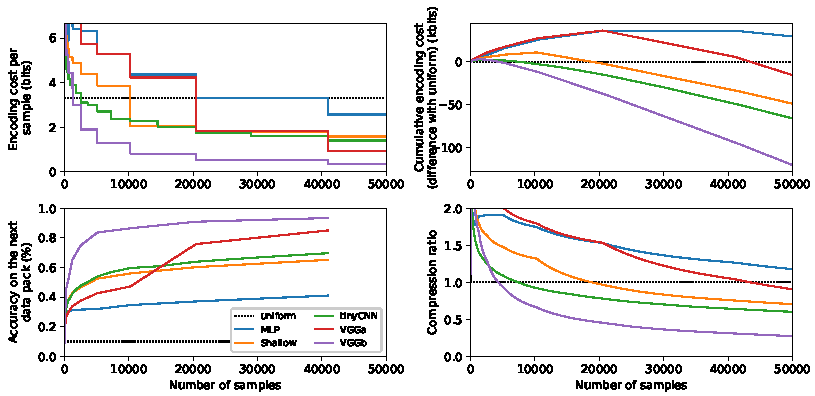
\includegraphics[width=\linewidth]{fig2_prequential_cifar}
    \end{column}
    \begin{column}{0.38\textwidth}
      \footnotesize
      \textcolor{structure}{Что на графиках} (ось $x$ --- сколько примеров уже передано):
      \begin{itemize}
        \item слева: бит на пример и точность на следующем блоке;
        \item справа: накопленная длина минус равномерный код (кбит) и коэффициент сжатия на $[1;t_k]$.
      \end{itemize}
      \textcolor{structure}{Что видно}
      \begin{itemize}
        \item лучше всех VGGb: 45,3 кбит (0,27);
        \item MLP на рисунке не опускается ниже равномерного кода;
        \item VGGa и VGGb --- одна архитектура, разная процедура обучения, разная длина кода.
      \end{itemize}
    \end{column}
  \end{columns}
\end{frame}

%% 11 --------------------------------------------------------------
\begin{frame}{Catch-up и переключение между моделями}
  \begin{columns}[T]
    \begin{column}{0.47\textwidth}
      \small
      \textcolor{structure}{Catch-up} (Van Erven et al., 2012): большая сеть переобучается на первых маленьких блоках и кодирует их хуже равномерного кода. VGGb: бит на пример ниже равномерного уже после 1000 примеров, а накопленное сжатие $<1$ только после 5000.

      \medskip
      \textcolor{structure}{Switch}: на каждом блоке кодируем лучшей моделью из \{uniform, tinyCNN, VGGa, VGGb\}; последовательность переключений $s$ передаётся за $-\log_2\pi(s)$ бит, это пренебрежимо мало.

      \medskip
      \textcolor{structure}{Self-switch}: одна архитектура, выбираем число эпох $j\le10$ на каждом блоке --- ранняя остановка как выбор модели.
    \end{column}
    \begin{column}{0.51\textwidth}
      \centering
      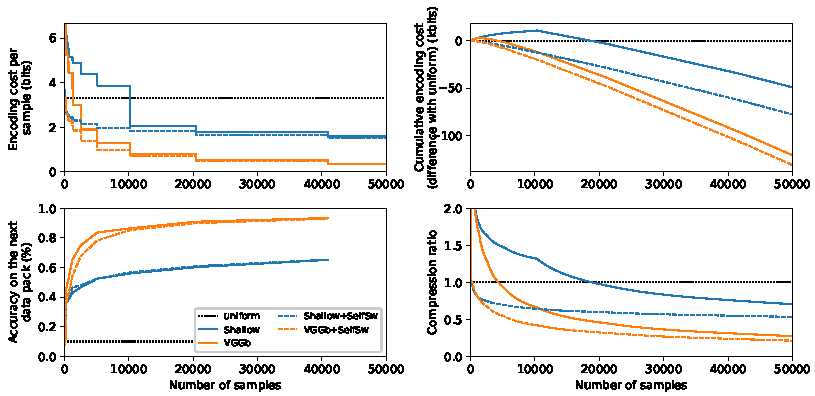
\includegraphics[width=\linewidth]{fig3_selfswitch_cifar}
      \footnotesize
      \begin{tabular}{lcc}
        \toprule
        Код (табл.~2) & MNIST, кбит & CIFAR-10, кбит \\
        \midrule
        Prequential & 4,10 & 45,3 (0,27) \\
        Switch & 4,05 & \textbf{34,6} (0,21) \\
        Self-switch & 4,05 & 34,9 (0,21) \\
        \bottomrule
      \end{tabular}
    \end{column}
  \end{columns}
\end{frame}

%% 12 --------------------------------------------------------------
\begin{frame}{Почему это неожиданно: в теории коды эквивалентны}
  \begin{block}{Классическая асимптотика (Grünwald, 2007)}
    \small Если модель $d$-мерная и идентифицируемая, данные порождены ею самой, prior подходящий, а эффективная размерность обученной модели не меньше $d$, то двухчастный, байесовский и prequential-код (на оценке ML или MAP) асимптотически эквивалентны:
    \[
      L(\yx)=nH(Y\mid X)+\frac d2\log_2n+O(1)\qquad\text{--- критерий BIC.}
    \]
  \end{block}
  \begin{itemize}\small
    \item Поэтому заранее не было причин ждать, что prequential-код окажется на порядок лучше.
    \item Глубокие сети не удовлетворяют \emph{ни одному} из этих условий.
    \item Prequential-код строится не на ML-оценке, а на обучении с регуляризацией (dropout, ранняя остановка).
  \end{itemize}
  \begin{alertblock}{Вывод авторов}
    С точки зрения теории информации \emph{число параметров само по себе не мешает сжатию} (гипотеза Чейтина: <<понимание --- это сжатие>>).
  \end{alertblock}
\end{frame}

%% 13 --------------------------------------------------------------
\begin{frame}{Почему вариационный код проигрывает: открытый вопрос}
  Вариационные методы плохи \emph{даже по собственному критерию} --- длине описания. Зазор до байесовского кода --- стандартное тождество ELBO:
  \[
    L^{\mathrm{var}}_\beta=L^{\mathrm{Bayes}}+\KL\big(\beta\,\big\|\,p_{\mathrm{Bayes}}(\theta\mid x_{1:n},y_{1:n})\big)
  \]
  \medskip
  \textcolor{structure}{Возможные причины по авторам}
  \begin{enumerate}
    \item Оптимизация параметров $\beta$ несовершенна.
    \item Даже лучшее $\beta^*$ из класса (диагональная гауссиана) плохо приближает апостериорное распределение, и KL велик.
    \item Prior, по мнению авторов, не главный фактор: гауссовы prior-ы с разной дисперсией и сопряжённый гауссов prior дали похожие результаты.
    \item Сам точный байесовский код может быть длиннее prequential: недообучение параметрического байесовского вывода, catch-up, консерватизм байесовского выбора моделей.
  \end{enumerate}
  Наблюдение: минимум вариационной длины выбирает \emph{меньшие} сети, чем кросс-валидация, и они хуже на тесте.
\end{frame}

%% 14 --------------------------------------------------------------
\begin{frame}{Что получилось и где слабые места}
  \small
  \begin{columns}[T]
    \begin{column}{0.5\textwidth}
      \textcolor{structure}{Выводы авторов}
      \begin{itemize}
        \item Глубокие сети сжимают метки с учётом стоимости модели: до 0,02 от равномерного кода на MNIST и до 0,21 на CIFAR-10 (switch).
        \item Число параметров не мешает сжатию.
        \item Двухчастный код с float32 и практическое сжатие сетей длиннее равномерного кода.
        \item Вариационный код в 2--6 раз длиннее prequential-кода, а модели хуже на тесте; почему --- открытый вопрос.
      \end{itemize}
    \end{column}
    \begin{column}{0.5\textwidth}
      \textcolor{structure}{Ограничения}
      \begin{itemize}
        \item Только классификация на MNIST и CIFAR-10 ($K=10$).
        \item Длина prequential-кода зависит от алгоритма обучения: у VGGa и VGGb одна архитектура, но разная длина.
      \end{itemize}
    \end{column}
  \end{columns}
\end{frame}

%% 15 --------------------------------------------------------------
\begin{frame}{Литература}
  \scriptsize
  \begin{thebibliography}{99}
    \bibitem{blier} Blier L., Ollivier Y. \emph{The description length of deep learning models.} NIPS 2018.
    \bibitem{grunwald} Grünwald P. D. \emph{The Minimum Description Length Principle.} MIT Press, 2007.
    \bibitem{solomonoff} Solomonoff R. \emph{A formal theory of inductive inference.} Information and Control, 1964.
    \bibitem{hinton} Hinton G. E., van Camp D. \emph{Keeping neural networks simple by minimizing the description length of the weights.} COLT 1993.
    \bibitem{honkela} Honkela A., Valpola H. \emph{Variational learning and bits-back coding.} IEEE Trans.\ Neural Networks, 2004.
    \bibitem{graves} Graves A. \emph{Practical variational inference for neural networks.} NIPS 2011.
    \bibitem{blundell} Blundell C. et al. \emph{Weight uncertainty in neural networks.} ICML 2015.
    \bibitem{dawid} Dawid A. P. \emph{Statistical theory: the prequential approach.} JRSS A, 1984.
    \bibitem{vanerven} Van Erven T., Grünwald P., de Rooij S. \emph{Catching up faster by switching sooner.} JRSS B, 2012.
    \bibitem{zhang} Zhang C. et al. \emph{Understanding deep learning requires rethinking generalization.} ICLR 2017.
    \bibitem{li} Li C. et al. \emph{Measuring the intrinsic dimension of objective landscapes.} 2018.
    \bibitem{han} Han S., Mao H., Dally W. J. \emph{Deep compression: compressing deep neural networks with pruning, trained quantization and Huffman coding.} 2015.
  \end{thebibliography}
\end{frame}

%% 16 --------------------------------------------------------------
\begin{frame}{Два вопроса к аудитории}
  \begin{enumerate}
    \setlength{\itemsep}{1.2em}
    \item Почему в prequential-коде не нужно передавать веса сети и что Алиса и Боб должны согласовать заранее?
    \item Сеть выучила случайные метки до 100\% точности на обучающей выборке. Почему эти метки всё равно нельзя сжать?
  \end{enumerate}
  \vfill
  \centering\Large Спасибо за внимание!
\end{frame}

\end{document}
